\chapter{实证结果与分析}\label{chap:4}
\section{描述性统计}

表\ref{tab:desc}报告了变量的描述性统计结果。本研究收集了522,085个观测值,描述性统计分析结果显示,保额Coverage的均值为514,139.56元,保费Premium的均值为1,175.71元,保险标的购置价Price均值为0.61百万元。是否此前投保(Prem\_before)的均值为0.04,标准差为0.20,显示第一次投保的比例较高。监测站点和保单的地理位置距离(distance)的均值为13.24,标准差为4.46,表明观测点之间的距离相对集中。累计降水量(累计降水量)的均值为2,042.35,标准差为712.30,显示了不同观测点之间降水量的变异性。
% 表\ref{tab:corr}报告了主要变量的相关系数矩阵,变量相关系数极低,说明本文的实证研究结果不存在多重共线性。

\begin{table}[H]
    \caption{数据描述性统计}\label{tab:desc}
    \centering
    \begin{tabular}{lrrrrrr}
\toprule
 & 观测数 & 均值 & 标准差 & 最小值 & 中位数 & 最大值 \\
\midrule
Coverage & 741442 & 288407.75 & 318090.33 & 20092.78 & 192000.00 & 2991900.00 \\
Disaster & 741442 & 0.12 & 0.32 & 0 & 0 & 1 \\
Neighbor & 741442 & 0.04 & 0.20 & 0 & 0 & 1 \\
Post & 741442 & 0.88 & 0.33 & 0 & 1 & 1 \\
Price & 741442 & 47.26 & 49.75 & 0 & 30.50 & 371.07 \\
GDP & 741442 & 8422.33 & 11370.88 & 0.07 & 0.25 & 49110.27 \\
Density & 741442 & 224.97 & 152.41 & 39.47 & 183.02 & 821.75 \\
Penetration & 741442 & 0.78 & 0.17 & 0.45 & 0.79 & 1.20 \\
Prem\_before & 741442 & 0.03 & 0.16 & 0 & 0 & 1 \\
Claim & 741442 & 0 & 0.04 & 0 & 0 & 1 \\
Premium & 741442 & 1014.95 & 1025.45 & 10.20 & 650.00 & 5558.00 \\
累计赔付额 & 741442 & 33.77 & 2741.24 & 0 & 0 & 517183.53 \\
保费 & 741442 & 1014.95 & 1025.45 & 10.20 & 650.00 & 5558.00 \\
累计降水量 & 741442 & 1474.29 & 1090.56 & 0 & 1721.00 & 6203.00 \\
\bottomrule
\end{tabular}

\end{table}

% \begin{table}[H]
%     \caption{变量之间相关性}\label{tab:corr}
%     \centering
%     \begin{tabular}{lrrrrrrr}
\toprule
 & Coverage & Disaster & Neighbor & Post & Prem\_before & Price & Area \\
\midrule
Coverage & 1.000000 & -0.003438 & 0.002232 & 0.006549 & 0.049063 & 0.195955 & -0.000131 \\
Disaster & -0.003438 & 1.000000 & -0.112619 & -0.199710 & -0.031179 & -0.027510 & -0.000619 \\
Neighbor & 0.002232 & -0.112619 & 1.000000 & -0.025723 & 0.004791 & 0.002799 & -0.000466 \\
Post & 0.006549 & -0.199710 & -0.025723 & 1.000000 & 0.014869 & 0.023873 & 0.000746 \\
Prem\_before & 0.049063 & -0.031179 & 0.004791 & 0.014869 & 1.000000 & 0.080722 & -0.000330 \\
Price & 0.195955 & -0.027510 & 0.002799 & 0.023873 & 0.080722 & 1.000000 & -0.000173 \\
Area & -0.000131 & -0.000619 & -0.000466 & 0.000746 & -0.000330 & -0.000173 & 1.000000 \\
\bottomrule
\end{tabular}


% \end{table}

\section{计量结果}
% \subsection{模型\ref{eq:OLS}:基础回归}
% 对于假设H\ref{hyp:1},回归结果见表\ref{tab:ols}。

% \begin{table}[htbp]
%     \centering
%     \caption{OLS回归结果}\label{tab:ols}
%     
\begin{tabular}{@{\extracolsep{5pt}}lcc}
\\[-1.8ex]\hline
\hline \\[-1.8ex]
& \multicolumn{2}{c}{\textit{Dependent variable: log(Coverage)}} \
\cr \cline{2-3}
\\[-1.8ex] & (1) & (2) \\
\hline \\[-1.8ex]
 Area & & -0.000$^{}$ \\
& & (0.000) \\
 Intercept & 12.265$^{***}$ & 12.158$^{***}$ \\
& (0.004) & (0.003) \\
 Post & 0.100$^{***}$ & 0.071$^{***}$ \\
& (0.004) & (0.004) \\
 Prem\_before & & 0.670$^{***}$ \\
& & (0.008) \\
 Price & & 0.136$^{***}$ \\
& & (0.001) \\
\hline \\[-1.8ex]
 Observations & 414961 & 414961 \\
 $R^2$ & 0.001 & 0.171 \\
 Adjusted $R^2$ & 0.001 & 0.171 \\
 Residual Std. Error & 1.021 (df=414959) & 0.930 (df=414956) \\
 F Statistic & 584.020$^{***}$ (df=1; 414959) & 21392.415$^{***}$ (df=4; 414956) \\
\hline
\hline \\[-1.8ex]
\textit{Note:} & \multicolumn{2}{r}{$^{*}$p$<$0.1; $^{**}$p$<$0.05; $^{***}$p$<$0.01} \\
\end{tabular}

% \end{table}

\subsection{模型\ref{eq:DID_1}:近灾区与远灾区DID回归}
对于假设H\ref{hyp:3},回归结果见表\ref{tab:did1}。回归结果显示,在控制了其他变量之后,当极端天气事件发生(即$\text{Post=1}$)时,不论家庭是否直接受灾或其居住地是否靠近灾区,家财险的保额整体上提高了约7\%。这一提升是显著为正,意味着在极端天气事件的影响下,家庭的风险感知得到了加强,从而增加了他们对家财险的需求。这一发现与假设H\ref{hyp:1}的预期一致,即极端天气事件通过提高风险感知,导致家财险需求的提升。

控制变量方面,回归结果还表明,保险标的的购置价每提升100万元导致保额平均提升15\%,家庭之前投保过会导致保额平均提升54\%。这两个变量的系数显著为正,与直觉相符,即价值较高的财和有保险购买历史的家庭更倾向于购买更高额度的保险。建筑面积对保额的影响较低,可能是因为家庭财产保险的保额不仅仅与建筑本身有关,还包括了其他与建筑无关但同样重要的物品,如家具、电器等。

此外,DID回归结果还揭示了近灾区与远灾区之间的差异。近灾区的系数显著为正,表明与远灾区相比,近灾区的居民在灾害发生后购买的家财险保额提升了约22\%。这一差异可能源于近灾区居民对极端降水概率的主观判断更高,因此他们的风险感知也更强。这种强烈的风险感知可能促使他们购买更高额度的保险,以更好地保护自己的财产。

最后,近灾区的交互项$\text{Neighbor}\times \text{Post}$的系数同样显著为正,这一结果验证了假设H\ref{hyp:3},意味着在极端天气事件发生后,近灾区的保额提升了约9\%。近灾区居民由于接收到更丰富的信息,对极端天气事件的敏感度增强,因此他们的保险需求也相应增加。这种信息的丰富性可能来自于更直接的灾害经历、媒体报道、社区讨论等多种渠道,使得近灾区居民对灾害的潜在影响有了更深刻的认识。

\begin{table}[htbp]
    \centering
    \caption{实验组为近灾区的DID回归结果}\label{tab:did1}
    
\begin{tabular}{@{\extracolsep{5pt}}lcc}
\\[-1.8ex]\hline
\hline \\[-1.8ex]
& \multicolumn{2}{c}{\textit{Dependent variable: log(Coverage)}} \
\cr \cline{2-3}
\\[-1.8ex] & (1) & (2) \\
\hline \\[-1.8ex]
 Area & & -0.000$^{}$ \\
& & (0.000) \\
 Intercept & 12.164$^{***}$ & 12.067$^{***}$ \\
& (0.005) & (0.004) \\
 Neighbor & 0.227$^{***}$ & 0.224$^{***}$ \\
& (0.013) & (0.012) \\
 Neighbor:Post & 0.086$^{***}$ & 0.087$^{***}$ \\
& (0.015) & (0.014) \\
 Post & 0.095$^{***}$ & 0.068$^{***}$ \\
& (0.005) & (0.005) \\
 Prem\_before & & 0.542$^{***}$ \\
& & (0.008) \\
 Price & & 0.153$^{***}$ \\
& & (0.001) \\
\hline \\[-1.8ex]
 Observations & 455107 & 455107 \\
 $R^2$ & 0.006 & 0.136 \\
 Adjusted $R^2$ & 0.006 & 0.136 \\
 Residual Std. Error & 1.150 (df=455103) & 1.072 (df=455100) \\
 F Statistic & 961.465$^{***}$ (df=3; 455103) & 11948.789$^{***}$ (df=6; 455100) \\
\hline
\hline \\[-1.8ex]
\textit{Note:} & \multicolumn{2}{r}{$^{*}$p$<$0.1; $^{**}$p$<$0.05; $^{***}$p$<$0.01} \\
\end{tabular}

\end{table}

\subsection{模型\ref{eq:DID_2}:灾区与远灾区DID回归}
对于假设H\ref{hyp:2},回归结果见表\ref{tab:did2}。与表\ref{tab:did1}类似,该组也验证了假设H\ref{hyp:1},即极端天气事件发生后购买家财险的保额提升约7\%;与表\ref{tab:did1}类似,该组也验证了假设H\ref{hyp:3},即灾区由于极端天气发生频率高,风险感知更强,在极端天气发生前的保额相对更高约20\%。但是,交互项$\text{Disaster}\times \text{Post}$的系数为负,即灾区相对非灾区在受灾后反而降低了30\%保额,几乎抵消了受灾后的20\%保额增加的影响,也就是几乎没有增加保额。
\begin{table}[htbp]
    \centering
    \caption{实验组为灾区的DID回归结果}\label{tab:did2}
    
\begin{tabular}{@{\extracolsep{5pt}}lcc}
\\[-1.8ex]\hline
\hline \\[-1.8ex]
& \multicolumn{2}{c}{\textit{Dependent variable: log(Coverage)}} \
\cr \cline{2-3}
\\[-1.8ex] & (1) & (2) \\
\hline \\[-1.8ex]
 Area & & -0.000$^{}$ \\
& & (0.000) \\
 Disaster & 0.187$^{***}$ & 0.207$^{***}$ \\
& (0.009) & (0.008) \\
 Disaster:Post & -0.333$^{***}$ & -0.310$^{***}$ \\
& (0.011) & (0.010) \\
 Intercept & 12.164$^{***}$ & 12.071$^{***}$ \\
& (0.005) & (0.005) \\
 Post & 0.095$^{***}$ & 0.069$^{***}$ \\
& (0.005) & (0.005) \\
 Prem\_before & & 0.547$^{***}$ \\
& & (0.008) \\
 Price & & 0.144$^{***}$ \\
& & (0.001) \\
\hline \\[-1.8ex]
 Observations & 480733 & 480733 \\
 $R^2$ & 0.002 & 0.116 \\
 Adjusted $R^2$ & 0.002 & 0.116 \\
 Residual Std. Error & 1.163 (df=480729) & 1.095 (df=480726) \\
 F Statistic & 360.218$^{***}$ (df=3; 480729) & 10506.506$^{***}$ (df=6; 480726) \\
\hline
\hline \\[-1.8ex]
\textit{Note:} & \multicolumn{2}{r}{$^{*}$p$<$0.1; $^{**}$p$<$0.05; $^{***}$p$<$0.01} \\
\end{tabular}

\end{table}

在分析灾区保额在极端天气冲击后降低的现象时,我们可以从两个角度来探讨其可能的影响因素。一个是获得性启发理论\citep{0Do},从居民的心理预期角度来看,当灾区居民经历极端天气事件后,他们可能会重新评估灾害风险,发现实际的损失并没有达到预期的严重程度。这种认知上的变化可能导致他们认为高额的保险投保并不必要,因此选择降低保险额度,以减少未来的保险费用支出。这种心理预期的调整可能是由于居民对灾害的直观感受和对保险赔付能力的初步判断所驱动的。另一个视角是保险公司的逆向选择,从保险市场的运作机制来看,灾区居民可能通过观察和经验发现,保险公司在灾害发生后的赔付比较有限,这可能是由于保险公司巨灾后的赔付策略、资金流动性或风险控制等多种因素造成的\citep{田玲2009中国财产保险业巨灾损失赔付能力实证研究}。当居民意识到即使购买了保险,实际获得的赔付也可能远远低于预期,他们可能会认为保险的经济性不高,从而减少投保额度,以避免支付高额的保险费用而获得较低的保障。

为了深入理解这两种因素对灾区赔付的影响,本文采用DID进行Logit回归分析。回归的因变量之一是“是否理赔”($\text{Claims}$),即保单在灾害发生后是否获得了保险公司的赔付;另一个因变量是“是否续约”($\text{Renew}$),即保单持有者是否选择在第二年继续购买同一保险产品。通过比较灾害发生前后的保险行为变化,我们可以更准确地捕捉到灾害对保险市场的影响。

根据DID Logit回归的结果表\ref{tab:claims},续约的交互项系数为正,这表明在经历了极端天气事件后,灾区居民实际上更愿意续保,这可能是因为他们认识到了灾害风险的严重性。然而,与此同时,保险公司的赔付能力可能并未达到居民的期望,也即巨灾风险暴露与巨灾保险赔付存在不对称\citep{张旭升2010中国巨灾风险暴露与巨灾保险赔付不对称实证},导致他们在续保时选择降低投保额,以减少不必要的保险费用。这也解释了为什么在受灾前的续约系数显著为负,即在没有灾害发生的情况下,居民可能主要因为对保险赔付量的怀疑而不愿意续保。

\begin{table}[htbp]
    \centering
    \caption{灾区与非灾区赔付/续约DID回归结果}\label{tab:claims}
    
\begin{tabular}{@{\extracolsep{5pt}}lcccc}
\\[-1.8ex]\hline
\hline \\[-1.8ex]
\\[-1.8ex] & \multicolumn{1}{c}{Claim} & \multicolumn{1}{c}{Claim} & \multicolumn{1}{c}{Renew} & \multicolumn{1}{c}{Renew}  \\
\\[-1.8ex] & (1) & (2) & (3) & (4) \\
\hline \\[-1.8ex]
 Disaster & 0.405$^{**}$ & 0.391$^{**}$ & -3.773$^{***}$ & -3.706$^{***}$ \\
& (0.169) & (0.169) & (0.221) & (0.222) \\
 Disaster:Post & 0.630$^{***}$ & 0.622$^{***}$ & 2.243$^{***}$ & 2.232$^{***}$ \\
& (0.190) & (0.190) & (0.234) & (0.235) \\
 Intercept & -6.825$^{***}$ & -4.664$^{***}$ & -5.228$^{***}$ & -11.891$^{***}$ \\
& (0.166) & (0.675) & (0.053) & (0.169) \\
 Post & -0.167$^{}$ & -0.158$^{}$ & -0.556$^{***}$ & -0.525$^{***}$ \\
& (0.123) & (0.123) & (0.028) & (0.029) \\
 Prem\_before & -2.299$^{***}$ & -2.246$^{***}$ & 4.428$^{***}$ & 4.338$^{***}$ \\
& (0.708) & (0.709) & (0.020) & (0.020) \\
 log(Coverage) & & -0.212$^{***}$ & & 0.668$^{***}$ \\
& & (0.067) & & (0.015) \\
 log(GDP) & -0.001$^{}$ & -0.001$^{}$ & 0.013$^{***}$ & 0.013$^{***}$ \\
& (0.006) & (0.006) & (0.002) & (0.002) \\
 log(Penetration) & -0.645$^{***}$ & -0.551$^{***}$ & 2.541$^{***}$ & 2.448$^{***}$ \\
& (0.152) & (0.156) & (0.056) & (0.056) \\
 log(Price) & 0.013$^{}$ & 0.140$^{**}$ & 0.499$^{***}$ & 0.031$^{***}$ \\
& (0.030) & (0.061) & (0.011) & (0.010) \\
\hline \\[-1.8ex]
 Observations & 709271 & 709271 & 709271 & 709271 \\
 Pseudo $R^2$ & 0.012 & 0.013 & 0.368 & 0.377 \\
 Yera FE & True & True & True & True \\
\hline
\hline \\[-1.8ex]
\textit{Note:} & \multicolumn{4}{r}{$^{*}$p$<$0.1; $^{**}$p$<$0.05; $^{***}$p$<$0.01} \\
\end{tabular}

\end{table}

\section{稳健性检验}
\subsection{平行趋势检验}

为了验证DID实证结果的稳健性,需要进行平行趋势检验。表\ref{tab:robust}展示了平行趋势检验的结果,并可视化如图\ref{fig:robust}。本文分别将实验组设置为灾区和近灾区($\text{Treat}=\text{Disaster}$以及$\text{Treat}=\text{Disaster}\text{Neighbor}$),对极端天气事件发生前三个季度的保额进行回归。结果显示在绝大多数回归中,交互项的系数都不显著,这表明在极端天气事件发生前,实验组和对照组的保额水平基本是平行的,满足平行趋势假设,可以通过DID方法来估计极端天气事件对家财险需求的影响。唯一表现出显著性的部分是在灾区受灾前90天内(一个季度)的保额,这可能是因为20年一遇的极端降水往往是持续较久的,灾区居民达到20年一遇的门槛前已经开始感知到风险,从而提前购买了保险。

\begin{table}[htbp]
    \centering
    \caption{平行趋势检验}\label{tab:robust}
    
\begin{tabular}{@{\extracolsep{5pt}}lcc}
\\[-1.8ex]\hline
\hline \\[-1.8ex]
& \multicolumn{2}{c}{\textit{Dependent variable: log(Coverage)}} \
\cr \cline{2-3}
\\[-1.8ex] & \multicolumn{1}{c}{Disaster} & \multicolumn{1}{c}{Neighbor}  \\
\\[-1.8ex] & (1) & (2) \\
\hline \\[-1.8ex]
 Treated:C(Quarter)[T.-1] & -0.007$^{}$ & 0.008$^{}$ \\
& (0.015) & (0.042) \\
 Treated:C(Quarter)[T.-2] & -0.005$^{}$ & 0.020$^{}$ \\
& (0.015) & (0.040) \\
 Treated:C(Quarter)[T.-3] & -0.005$^{}$ & 0.017$^{}$ \\
& (0.014) & (0.041) \\
 Treated:C(Quarter)[T.0] & -0.124$^{***}$ & 0.233$^{***}$ \\
& (0.011) & (0.030) \\
 Treated:C(Quarter)[T.1] & -0.150$^{***}$ & 0.261$^{***}$ \\
& (0.013) & (0.030) \\
 Treated:C(Quarter)[T.2] & -0.153$^{***}$ & 0.259$^{***}$ \\
& (0.013) & (0.030) \\
 Treated:C(Quarter)[T.3] & -0.157$^{***}$ & 0.238$^{***}$ \\
& (0.013) & (0.030) \\
 Treated:C(Quarter)[T.4] & -0.163$^{***}$ & 0.250$^{***}$ \\
& (0.013) & (0.030) \\
C(Quarter)[T.-1] & -0.006$^{}$ & -0.006$^{}$ \\
& (0.009) & (0.009) \\
 C(Quarter)[T.-2] & -0.004$^{}$ & -0.004$^{}$ \\
& (0.009) & (0.009) \\
 C(Quarter)[T.-3] & -0.002$^{}$ & -0.002$^{}$ \\
& (0.009) & (0.009) \\
 C(Quarter)[T.0] & 0.091$^{***}$ & 0.095$^{***}$ \\
& (0.007) & (0.007) \\
 C(Quarter)[T.1] & 0.096$^{***}$ & 0.099$^{***}$ \\
& (0.007) & (0.007) \\
 C(Quarter)[T.2] & 0.097$^{***}$ & 0.101$^{***}$ \\
& (0.007) & (0.007) \\
 C(Quarter)[T.3] & 0.096$^{***}$ & 0.100$^{***}$ \\
& (0.007) & (0.007) \\
 C(Quarter)[T.4] & 0.101$^{***}$ & 0.105$^{***}$ \\
& (0.007) & (0.007) \\
 Treated & -0.002$^{}$ & -0.211$^{***}$ \\
& (0.010) & (0.029) \\
 Controls & True & True \\
 Intercept & 10.986$^{***}$ & 11.042$^{***}$ \\
& (0.007) & (0.007) \\
\hline \\[-1.8ex]
 Observations & 709271 & 654504 \\
 $R^2$ & 0.385 & 0.364 \\
 Adjusted $R^2$ & 0.385 & 0.364 \\
 Residual Std. Error & 0.661  & 0.677  \\
 F Statistic & 21157.483$^{***}$  & 17827.292$^{***}$  \\
\hline
\hline \\[-1.8ex]
\textit{Note:} & \multicolumn{2}{r}{$^{*}$p$<$0.1; $^{**}$p$<$0.05; $^{***}$p$<$0.01} \\
\end{tabular}

\end{table}

\begin{figure}[htbp]
    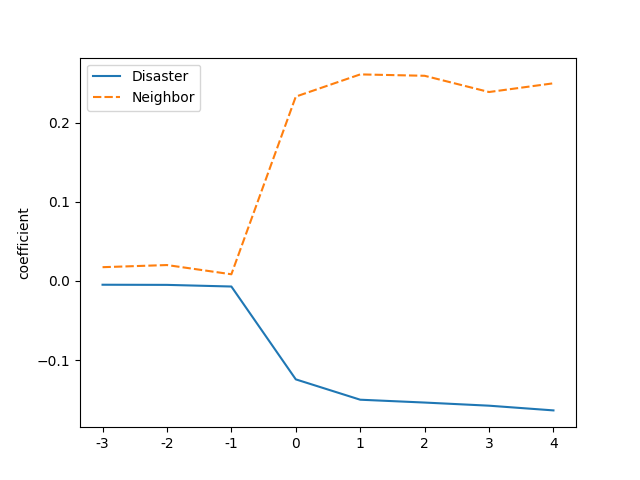
\includegraphics[width=\linewidth]{lib/img/robust.png}
    \caption{平行趋势检验}\label{fig:robust}
\end{figure}
\subsection{安慰剂检验}
为排除其他潜在政策和遗漏变量等对回归结果的干扰,本文参考\citet{CYJJ202104009}随机虚构处理组,将 Neighbor 和 Disaster 的 DID 随机分组分配重复 500 次,结果如图\ref{fig:randomtest}所示。随机分配结果的所有系数估计值大体呈均值为 0 的正态分布,说明实验结果不是由于其他潜在政策或遗漏变量引起的,而是由于极端天气事件的影响。
\begin{figure}[H]
    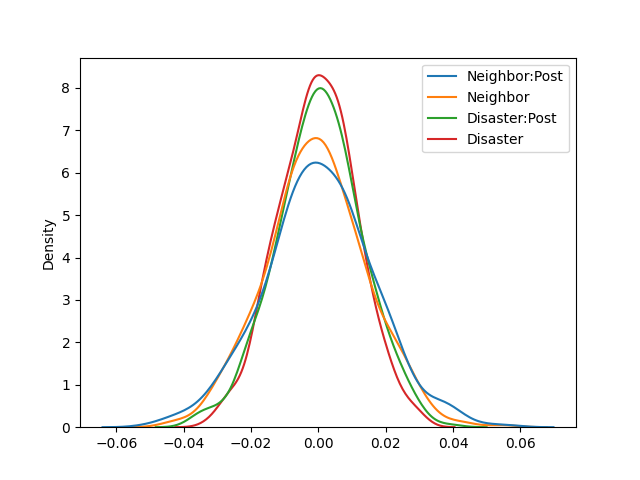
\includegraphics[width=\linewidth]{lib/img/randomtest.png}
    \caption{安慰剂检验}\label{fig:randomtest}
\end{figure}

\subsection{其他稳健性检验}

为保证基准回归结果的稳健性,本文还进行了以下稳健性检验:(1)(2)更换家财险需求的度量方式为保费Premium;(3)(4)/(5)(6)参考\citet{alok2020fund}分别将灾区距离上界从 20km 改为 30km 和 10km。回归结果如表\ref{tab:robustdid}所示。就回归结果而言,基本与基准回归结果一致,表明本文的实证结果是稳健的。这一结果进一步验证了极端天气事件通过增强家庭的风险感知,导致家财险需求的提升。
\begin{sidewaystable}[htbp]
    \centering
    \caption{分地区回归结果}\label{tab:robustdid}
    
\begin{tabular}{@{\extracolsep{5pt}}lcccccc}
\\[-1.8ex]\hline
\hline \\[-1.8ex]
\\[-1.8ex] & \multicolumn{1}{c}{log(Premium)} & \multicolumn{1}{c}{log(Premium)} & \multicolumn{1}{c}{<30km} & \multicolumn{1}{c}{<30km} & \multicolumn{1}{c}{<10km} & \multicolumn{1}{c}{<10km}  \\
\\[-1.8ex] & (1) & (2) & (3) & (4) & (5) & (6) \\
\hline \\[-1.8ex]
 Area & 0.000$^{}$ & 0.000$^{}$ & 0.000$^{}$ & 0.000$^{}$ & 0.000$^{}$ & 0.000$^{}$ \\
& (0.000) & (0.000) & (0.000) & (0.000) & (0.000) & (0.000) \\
 Disaster & & -0.149$^{***}$ & & 0.187$^{***}$ & & 0.170$^{***}$ \\
& & (0.009) & & (0.006) & & (0.011) \\
 Disaster:Post & & -0.036$^{***}$ & & -0.207$^{***}$ & & -0.277$^{***}$ \\
& & (0.011) & & (0.007) & & (0.013) \\
 Intercept & 6.257$^{***}$ & 6.255$^{***}$ & 12.052$^{***}$ & 12.055$^{***}$ & 12.086$^{***}$ & 12.106$^{***}$ \\
& (0.005) & (0.005) & (0.003) & (0.003) & (0.006) & (0.006) \\
 Neighbor & 0.065$^{***}$ & & 0.222$^{***}$ & & 0.158$^{***}$ & \\
& (0.013) & & (0.012) & & (0.014) & \\
 Neighbor:Post & 0.024$^{}$ & & 0.150$^{***}$ & & 0.209$^{***}$ & \\
& (0.015) & & (0.013) & & (0.016) & \\
 Post & 0.097$^{***}$ & 0.097$^{***}$ & -0.000$^{}$ & -0.000$^{}$ & 0.085$^{***}$ & 0.098$^{***}$ \\
& (0.005) & (0.005) & (0.003) & (0.003) & (0.002) & (0.002) \\
 Prem\_before & -0.801$^{***}$ & -0.785$^{***}$ & 0.574$^{***}$ & 0.576$^{***}$ & 0.386$^{***}$ & 0.395$^{***}$ \\
& (0.009) & (0.009) & (0.006) & (0.006) & (0.009) & (0.010) \\
 Price & 0.084$^{***}$ & 0.086$^{***}$ & 0.184$^{***}$ & 0.178$^{***}$ & 0.238$^{***}$ & 0.198$^{***}$ \\
& (0.001) & (0.001) & (0.001) & (0.001) & (0.001) & (0.001) \\
\hline \\[-1.8ex]
 Observations & 408439 & 433025 & 853757 & 939148 & 270762 & 277046 \\
 $R^2$ & 0.041 & 0.038 & 0.150 & 0.131 & 0.190 & 0.146 \\
 Adjusted $R^2$ & 0.041 & 0.038 & 0.150 & 0.131 & 0.190 & 0.146 \\
 Residual Std. Error & 1.138  & 1.143  & 1.076  & 1.098  & 1.022  & 1.065  \\
 F Statistic & 2885.524$^{***}$  & 2880.383$^{***}$  & 25027.608$^{***}$  & 23637.295$^{***}$  & 10588.824$^{***}$  & 7863.860$^{***}$  \\
\hline
\hline \\[-1.8ex]
\textit{Note:} & \multicolumn{6}{r}{$^{*}$p$<$0.1; $^{**}$p$<$0.05; $^{***}$p$<$0.01} \\
\end{tabular}

\end{sidewaystable}

具体而言,表\ref{tab:robustdid}的(1)(2)列显示,当极端天气事件发生后,家庭的保费整体上提高了约9\%。这一提升是显著为正,意味着在极端天气事件的影响下,家庭的风险感知得到了加强,从而增加了他们对家财险的需求。这一发现与假设H\ref{hyp:1}的预期一致,即极端天气事件通过提高风险感知,导致家财险需求的提升。但灾区交互项的系数为负,表明灾区的保费在受灾后反而降低了约3\%,近灾区则提升了约2\%,与假设H\ref{hyp:3}、假设H\ref{hyp:2}一致。

就更改距离而言,(3)(4)/(5)(6)分别更改灾区受灾半径的上界至10km/30km,整体而言并不会改变实证结果,同样显示出灾区灾后保额购买减少约20-30\%、近灾区保额购买提升15-20\%,表明本文的实证结果是稳健的。但当放大灾区半径到 30km 时,$\text{Post}$的系数变得不显著,这可能是因为灾区半径过大,受影响的地区被包含进了实验组,从而导致实验效果不显著。
